% -*- root: ../main.tex -*-
%Scelte rilevanti, pattern di progettazione, organizzazione del codice -- corredato da pochi ma efficaci diagrammi
%Il design di dettaglio "esplode" (dettaglia) l'architettura, ma viene concettualmente prima dell'implementazione, quindi non metteteci diagrammi ultra-dettagliati estratti dal codice, quelli vanno nella parte di implementazione eventualmente.
\chapter{Design di Dettaglio}\label{chap:design}
In questo capitolo, partendo dal design architetturale sopra descritto, verrà analizzata in dettaglio la struttura del sistema, descrivendo le caratteristiche dei componenti e la relazione che c'è tra loro.

    \section{Model}
        Il design del \textit{model} realizzato cerca di rispecchiare il dominio di questa applicazione in modo indipendente e generale rispetto all'implementazione che verrà eseguita successivamente. Il design dettagliato sarà di seguito esposto dividendolo in tre parti concettualmente separate. Essi riguardano rispettivamente gli elementi utilizzati durante una partita, quelli per il riepilogo e infine quelli relativi alla rappresentazione delle statistiche.
        
        \medskip
        L'elemento principale del \textit{model} utilizzato durante una partita è "GameStage", come già indicato in precedenza. Esso è contenuto nel \textit{controller}, ma a sua volta contiene tutti i componenti necessari per lo svolgimento di una generica partita:
        \begin{itemize}
            \item "GameSettings": rappresenta le impostazioni della partita e a sua volta si specializza per modellare le specifiche impostazioni relative ad una determinata modalità di gioco
            \item "Review": mantiene le informazioni riguardati lo svolgimento di una partita (verrà successivamente analizzato)
            \item "QuizInGame": modella il "Quiz", relativo ad uno specifico "Course", che viene proposto ad un utente in un particolare momento di gioco, comprensivo di una domanda e di alcune possibili "Answer"
            \item "CoursesInGame": rappresenta i "Course" selezionati tra i possibili "SavedCourse" da utilizzare per estrarre le domande da porre durante la partita
        \end{itemize}

        Come mostrato in Figura \ref{fig:model-game}, gli elementi base modellati nell'applicazione sono:
        \begin{itemize}
            \item "Course": descrive un corso universitario e presenta un identificativo, "CourseIdentifier", composto dal nome del corso, il nome dell'università in cui si svolge e la facoltà relativa. "Course" si specializza in "SavedCourse" fungendo da contenitore per un insieme di quiz salvati relativi al corso. 
            \item "Quiz": sono composti dal testo della domanda e da un insieme di possibili risposte associate. Sono contenuti in uno dei "SavedCourse" e contengono anche informazioni aggiuntive come, ad esempio, il punteggio del quiz.
            \item "Answer": modella una delle possibili risposte di un quiz ed è formata dal testo della risposta e da un'indicazione della correttezza di tale risposta.
        \end{itemize}
        
        \begin{figure}[H]
            \centering
            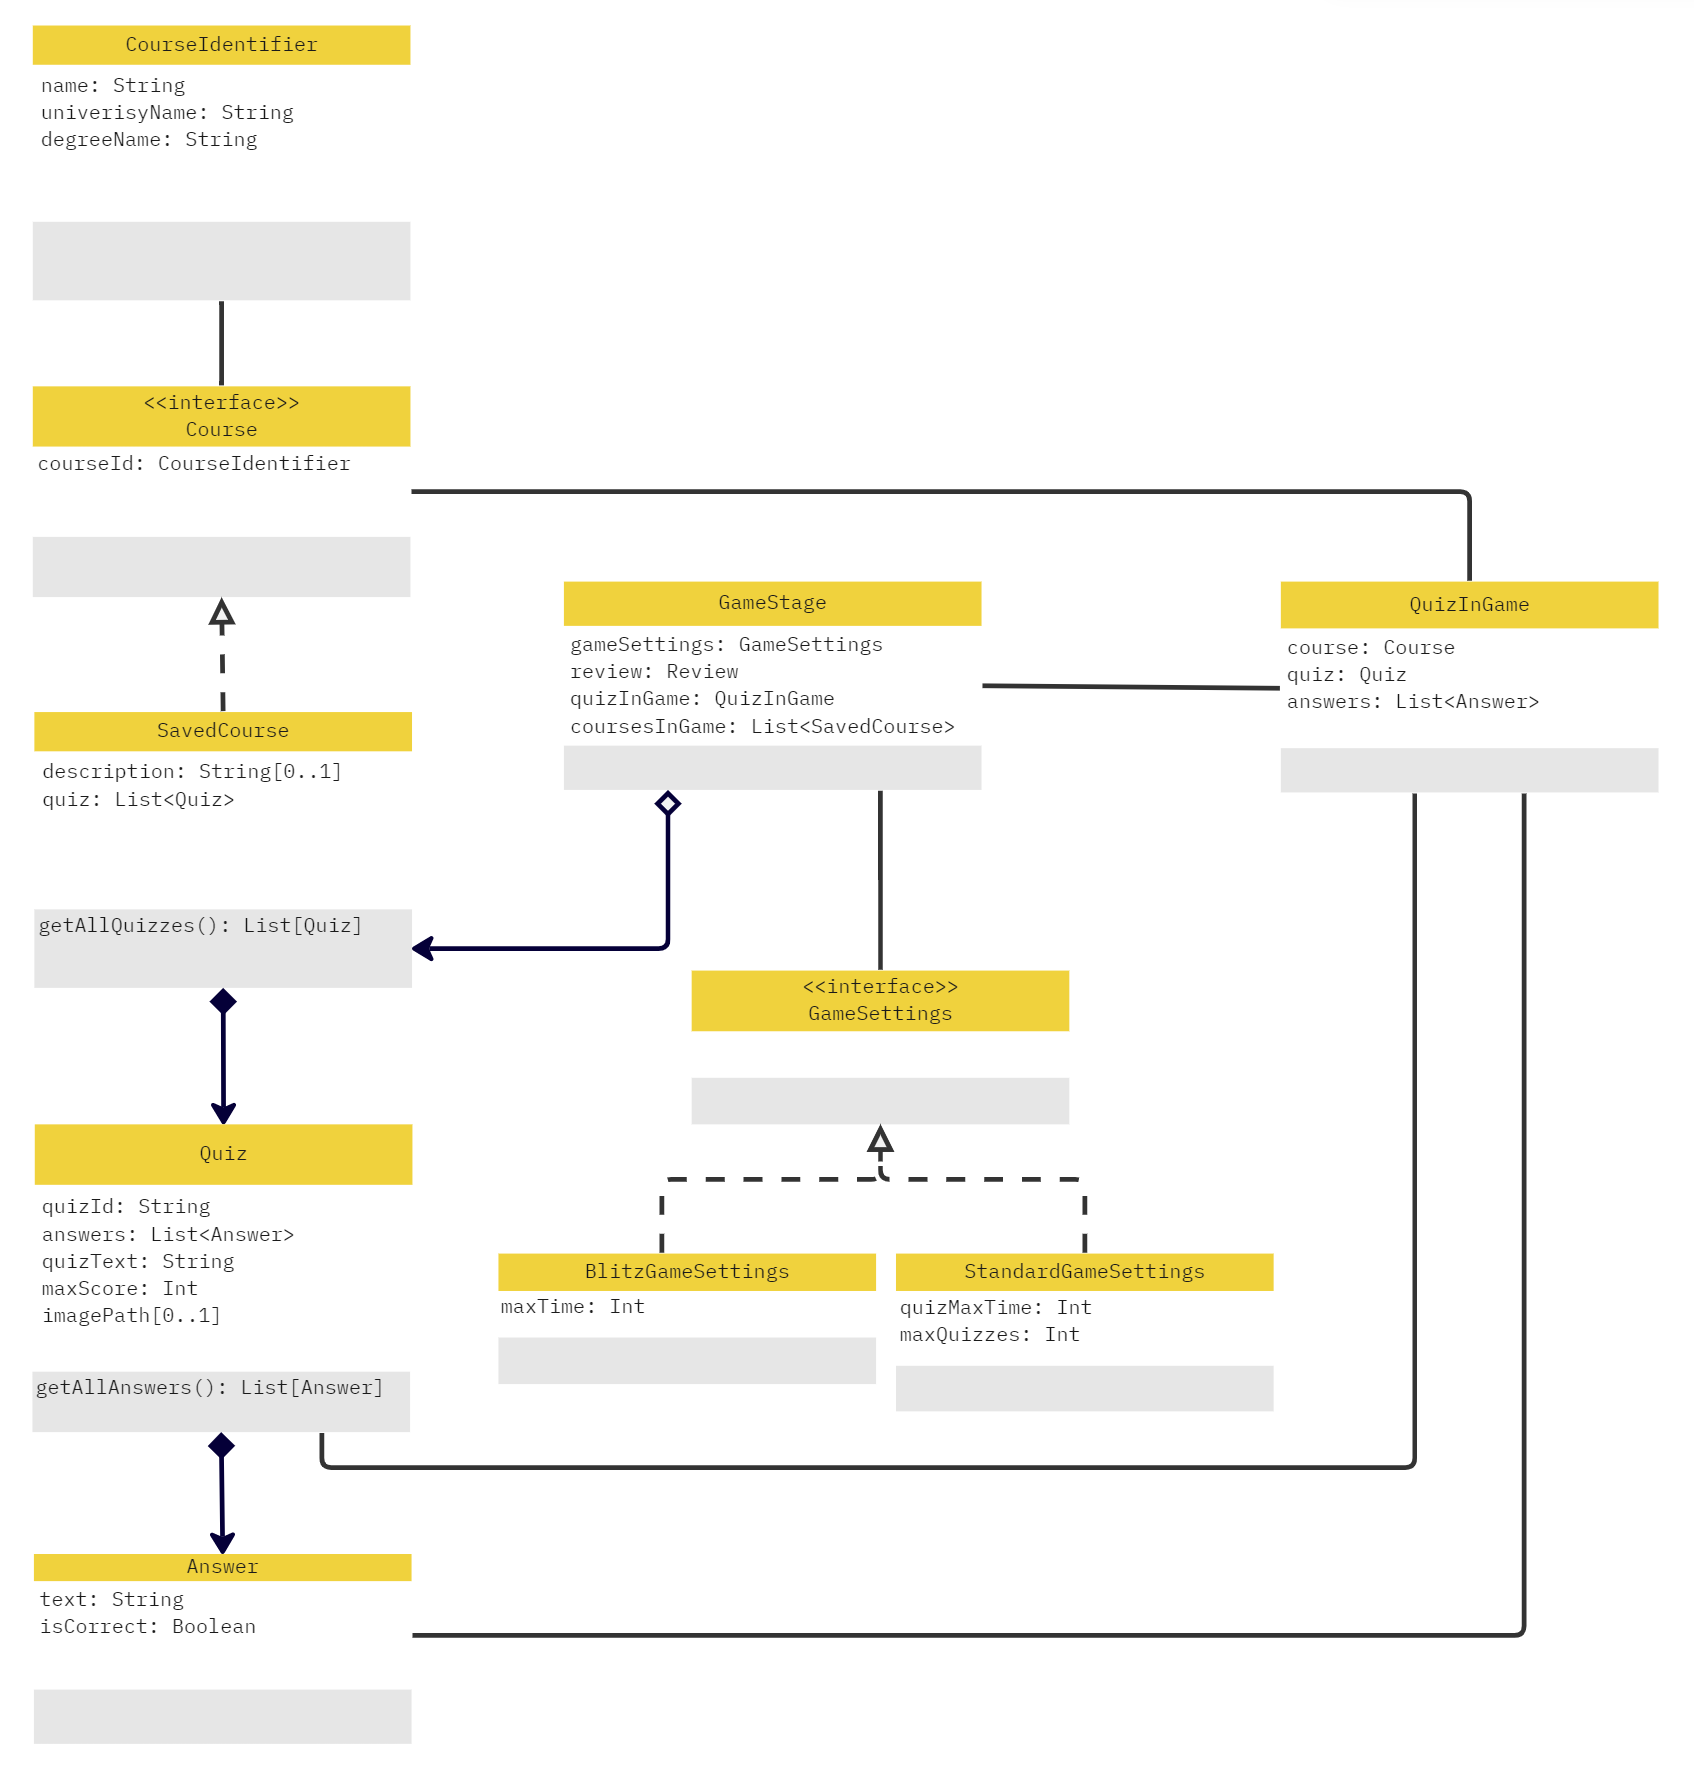
\includegraphics[scale=0.6]{Miro/game_model.png}
            \caption{Architettura del \textit{model} durante una partita}
            \label{fig:model-game}
        \end{figure}

        Come mostrato in Figura \ref{fig:model-review}, il riepilogo di una partita è contenuta nel "GameStage" e viene aggiornato durante la partita aggiungendo una serie di "QuizAnswered", ovvero i quiz che vengono posti all'utente durante lo svolgimento del gioco. "QuizAnswered" estende il "QuizInGame" con l'aggiunta della risposta scelta, il punteggio ottenuto e il tempo di risposta.
    
        \begin{figure}[H]
            \centering
            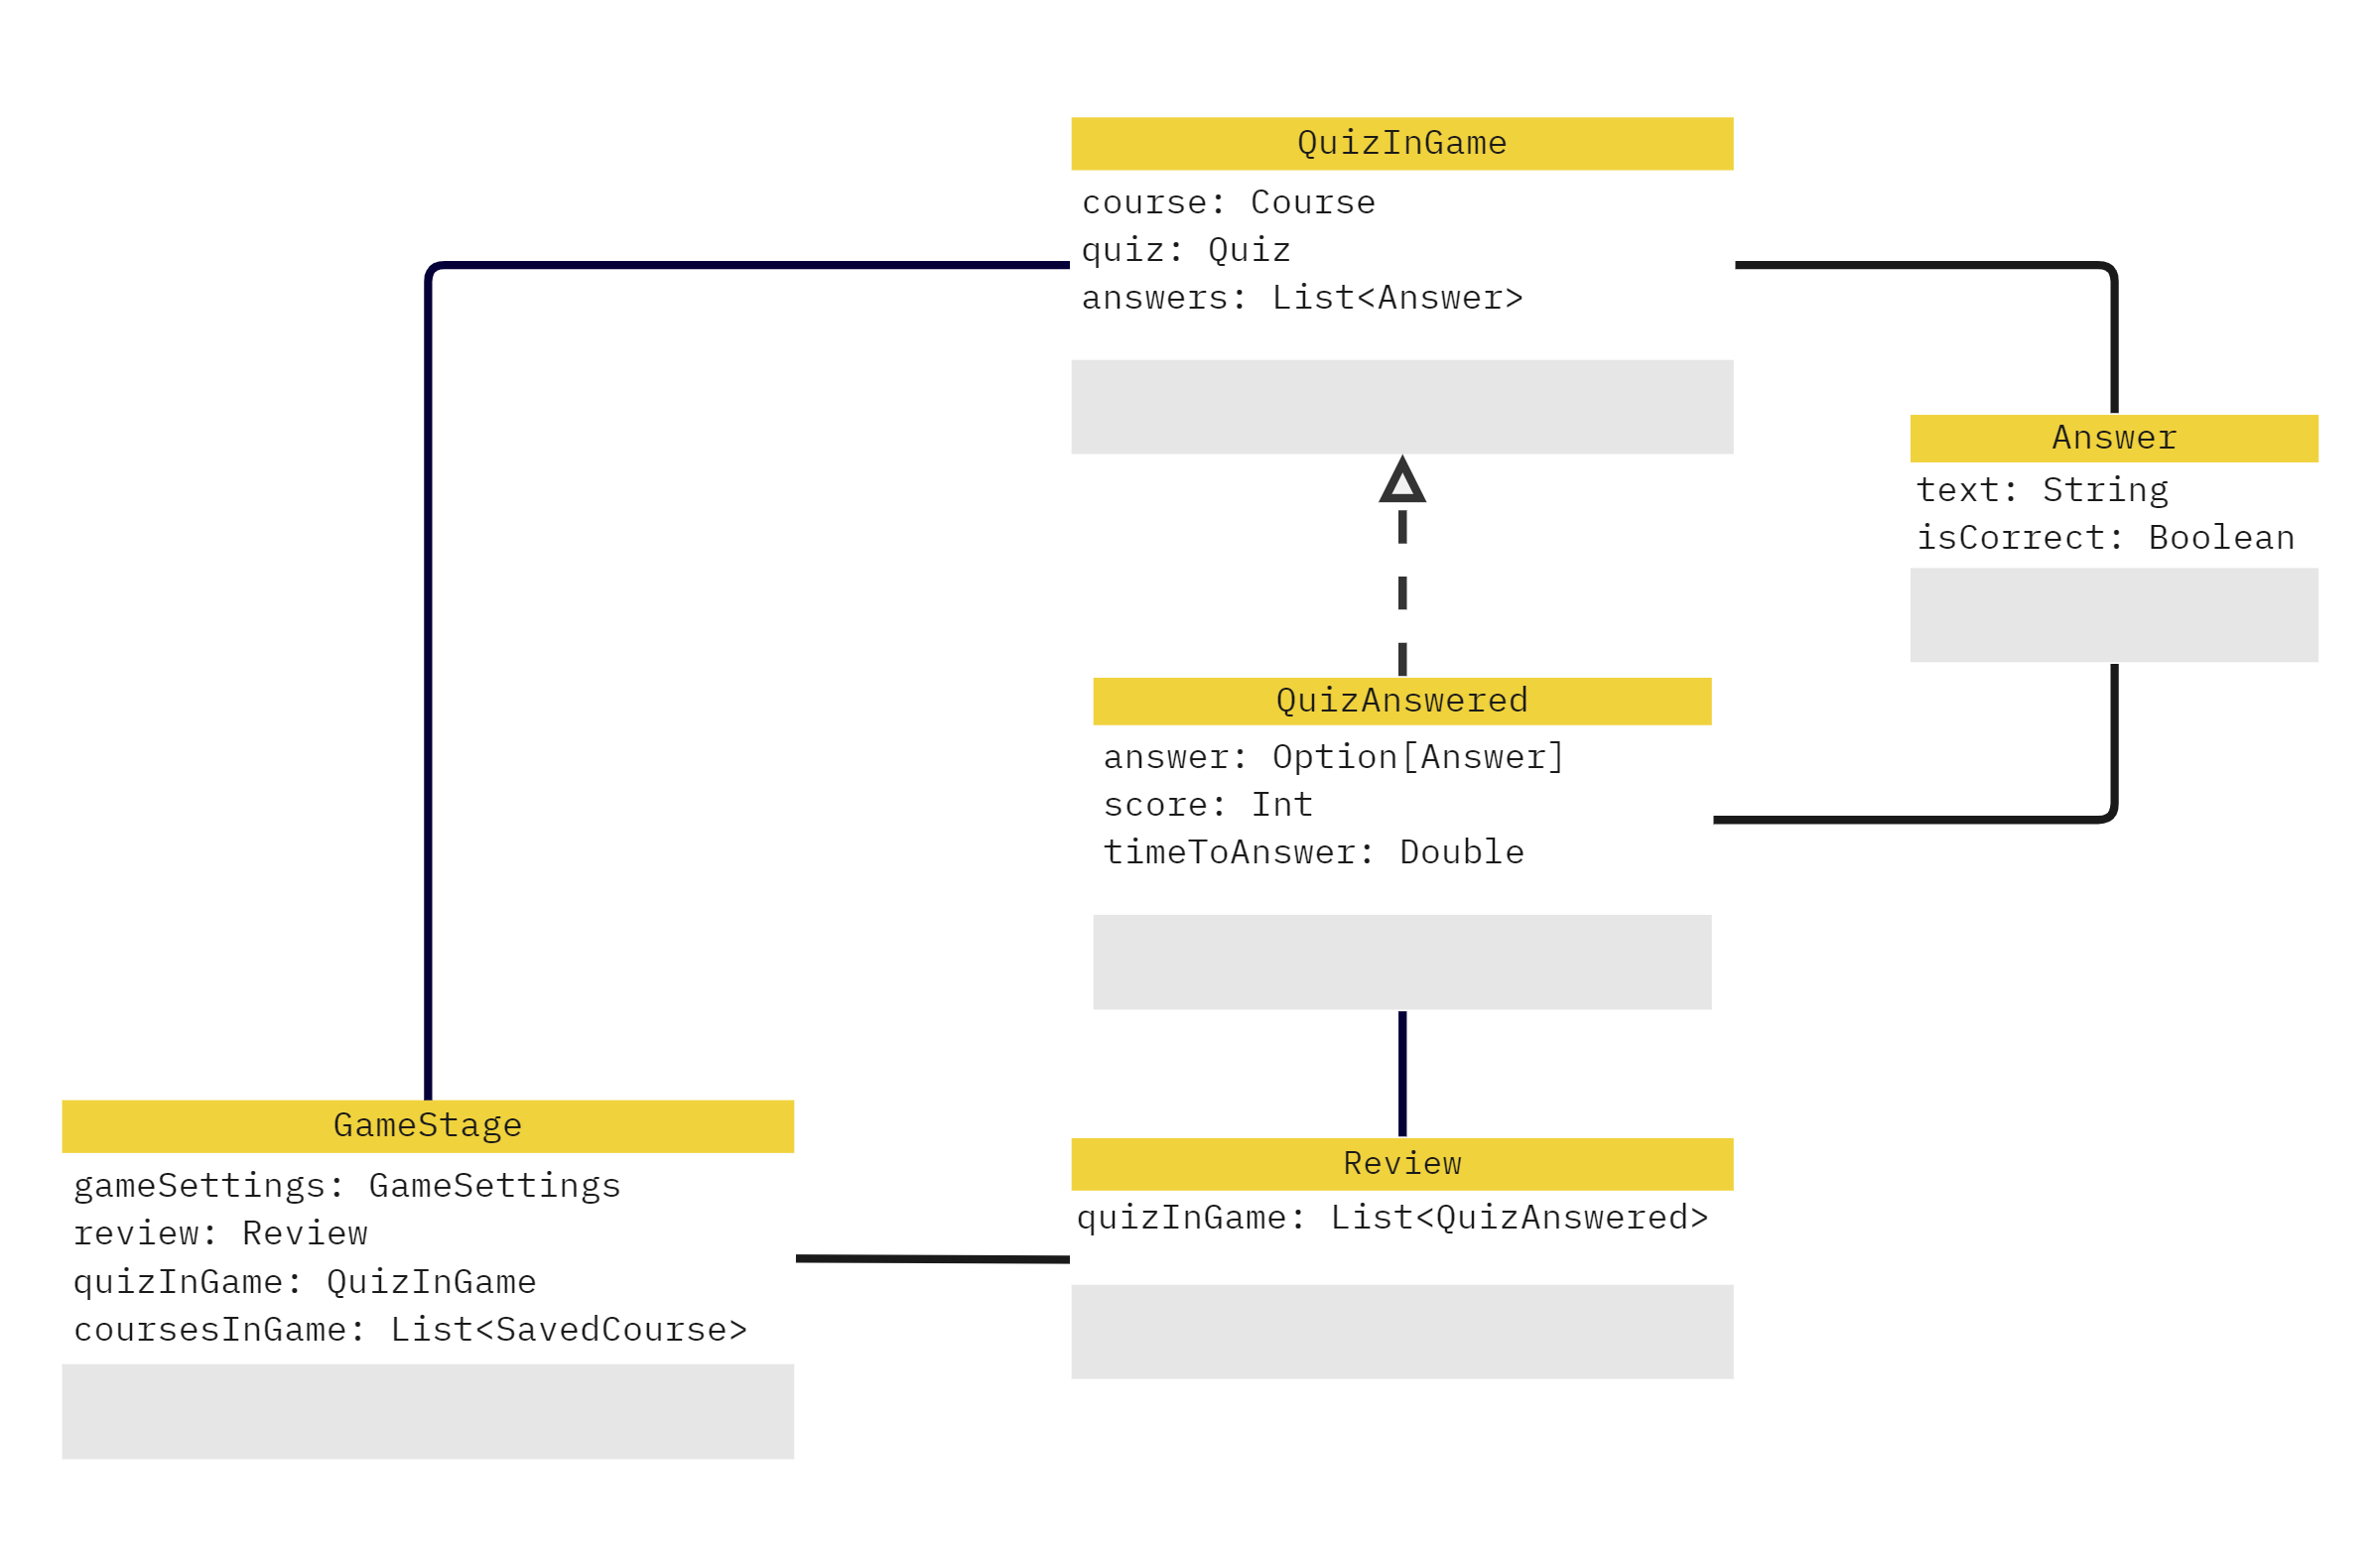
\includegraphics[scale=0.4]{Miro/review_model.png}
            \caption{Architettura del \textit{model} per il riepilogo}
            \label{fig:model-review}
        \end{figure}

        Per salvare i dati relativi alle statistiche di diverse partite, è stata realizzata una "Session", la quale viene aggiornata al termine di ogni partita con le nuove statistiche di gioco. Come si può vedere in Figura \ref{fig:model-statistics}, le statistiche mantengono una struttura dati su file simile a quella utilizzata per rappresentare i quiz e sono infatti modellate attraverso un "CourseInStat" con all'interno una serie di "QuizInStat". In questo modo viene mantenuta la struttura gerarchica tra quiz e corso, permettendo di ottenere eventualmente informazioni utili relative alle statistiche dei singoli quiz di un corso.

        \begin{figure}[H]
            \centering
            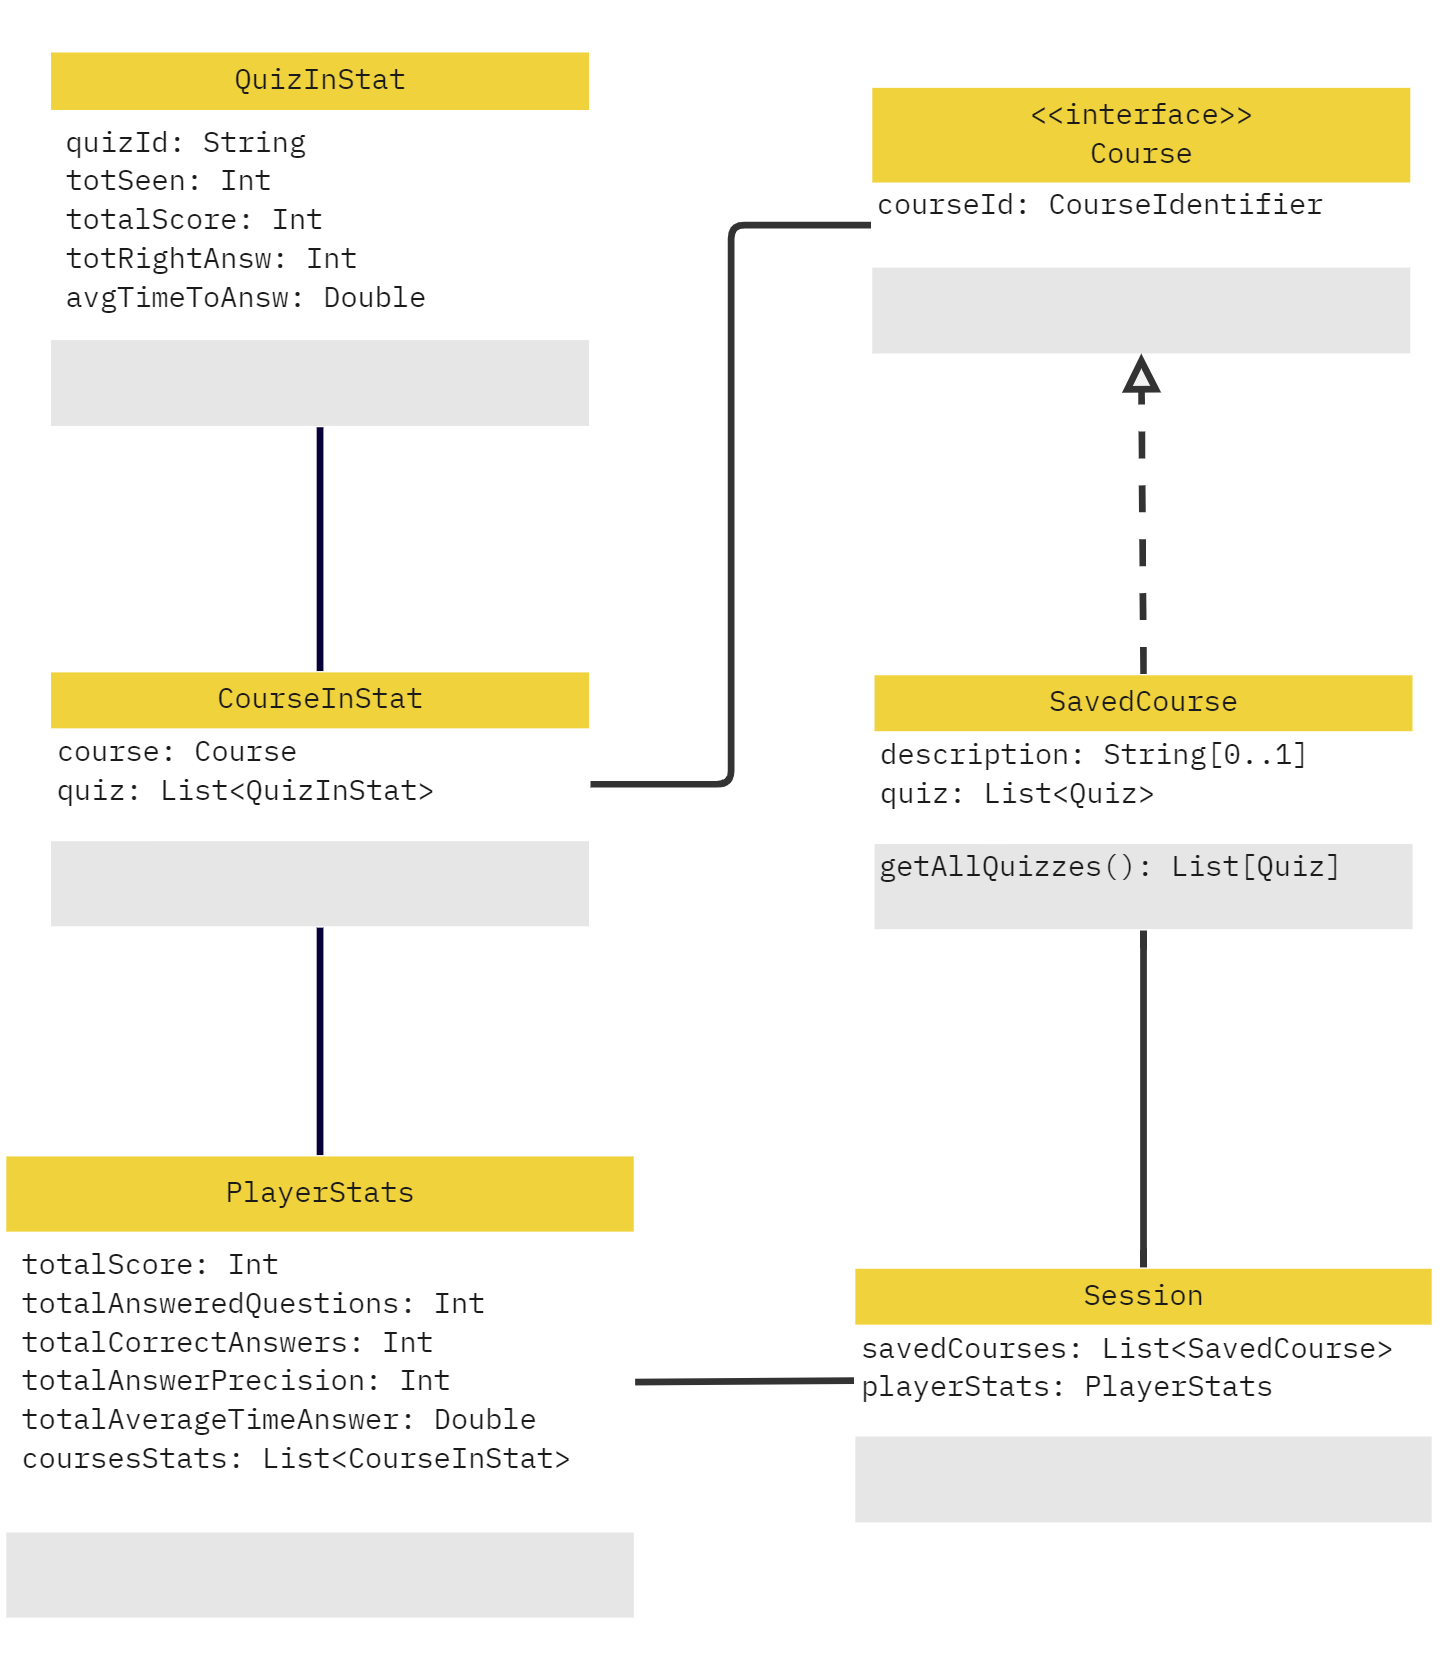
\includegraphics[scale=0.4]{Miro/statistics_model.png}
            \caption{Architettura del \textit{model} per le statistiche}
            \label{fig:model-statistics}
        \end{figure}
        
    \section{View}

    Come già spiegato nell'Architettura Generale \ref{chap:architectural-design} del sistema, ogni pagina dispone di una \textit{view} specifica. In Figura \ref{fig:view-dettaglio} sono mostrate come esempio le \textit{view} relative al menu di selezione dei corsi prima di una partita, "SelectMenuView", e quella di una partita standard, "StandardGameMenuView". Avendo utilizzato un processo di sviluppo agile, è stata inizialmente proposta all'esperto del dominio una versione dell'applicazione con interfaccia grafica tramite linea di comando. Tuttavia, il design della \textit{view} realizzato, è stato ideato in modo da rendere la view quanto più possibile indipendente dalla specifica implementazione. Infatti nelle fasi successive del progetto, quando è stata introdotta la GUI tramite JavaFX, è stato sufficiente realizzare la nuova implementazione rispettando le interfacce predisposte. Durante l'esecuzione dell'applicazione, la corretta implementazione della \textit{view} relativa ad una pagina viene instanziata attraverso una "ViewFactory" che restituisce la "PageView" corretta.
    
    \begin{figure}[H]
        \centering
        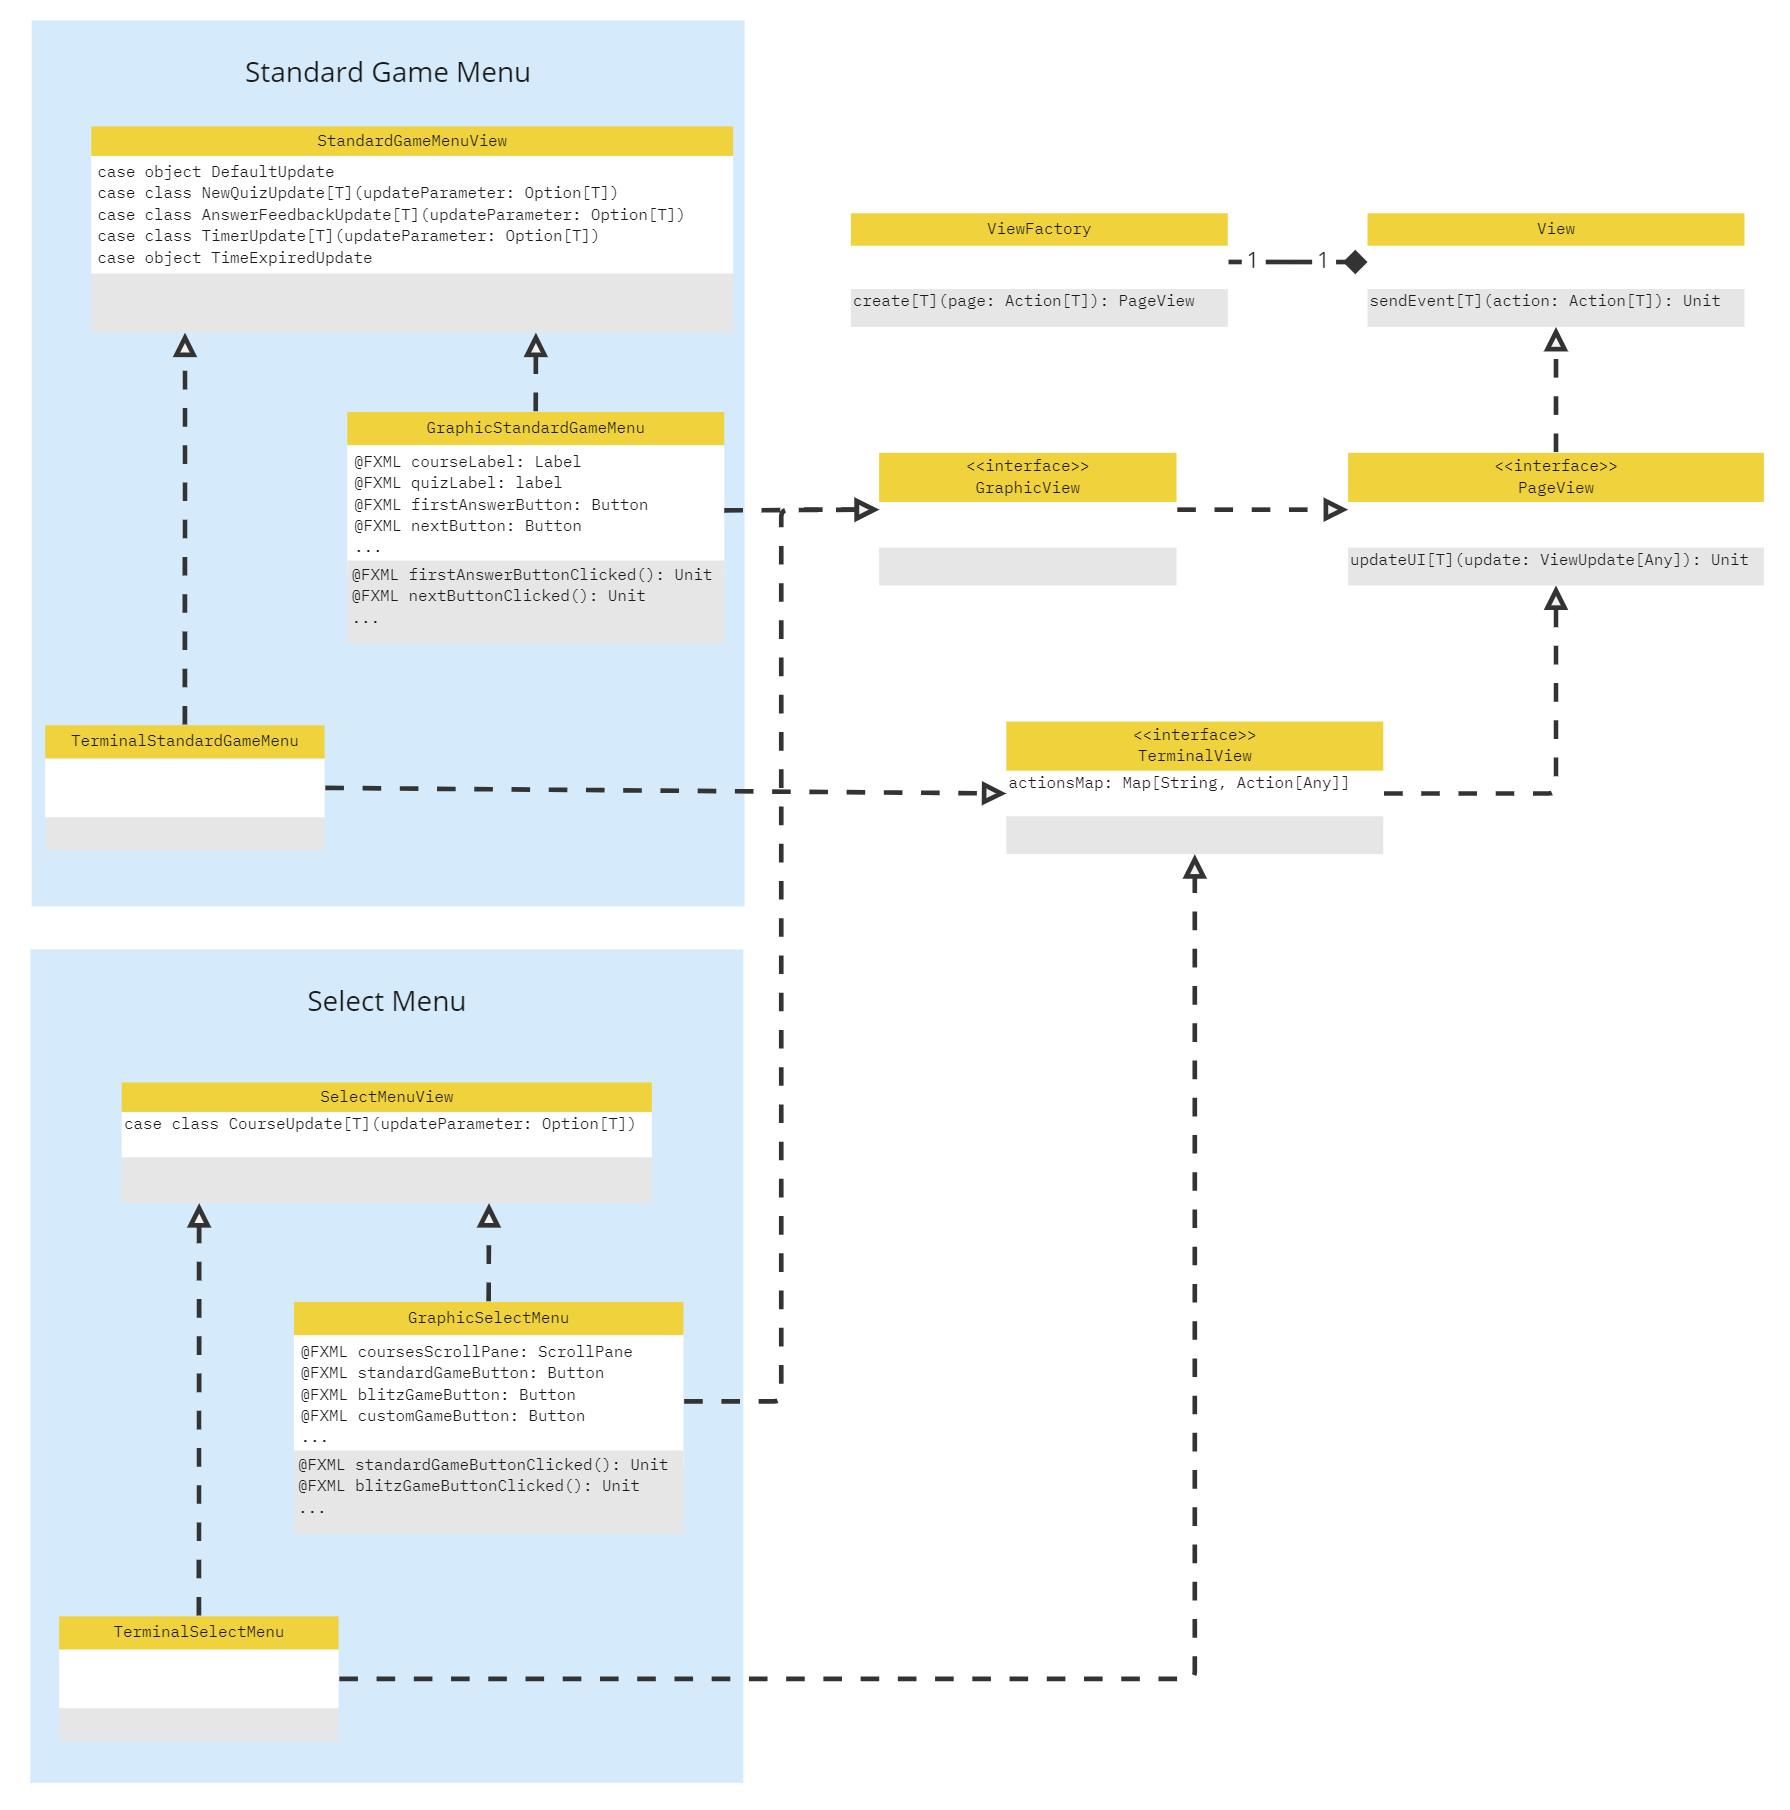
\includegraphics[width=\textwidth]{Miro/view.png}
        \caption{Architettura della \textit{view}}
        \label{fig:view-dettaglio}
    \end{figure}

    Ciascuna \textit{view} di una pagina mette a disposizione diversi "ViewUpdate" che è possibile richiamare per aggiornare alcuni degli elementi grafici. Gli updates della \textit{view} possono avere dei parametri generici e opzionali il cui valore costituisce le informazioni necessarie per effettuare l'aggiornamento (Figura \ref{fig:view-updates}). Nel caso uno degli update non necessiti di dati, è possibile utilizzare un "ParameterlessViewUpdate" il quale estende "ViewUpdate", definendo il parametro dell'aggiornamento come vuoto. Dato che tutte le interfacce grafiche delle pagine necessitano di un "DefaultUpdate", ovvero di un aggiornamento di base dell'interfaccia, esso è stato estratto in modo da evitare di definirlo molteplici volte.
    
    \begin{figure}[H]
        \centering
        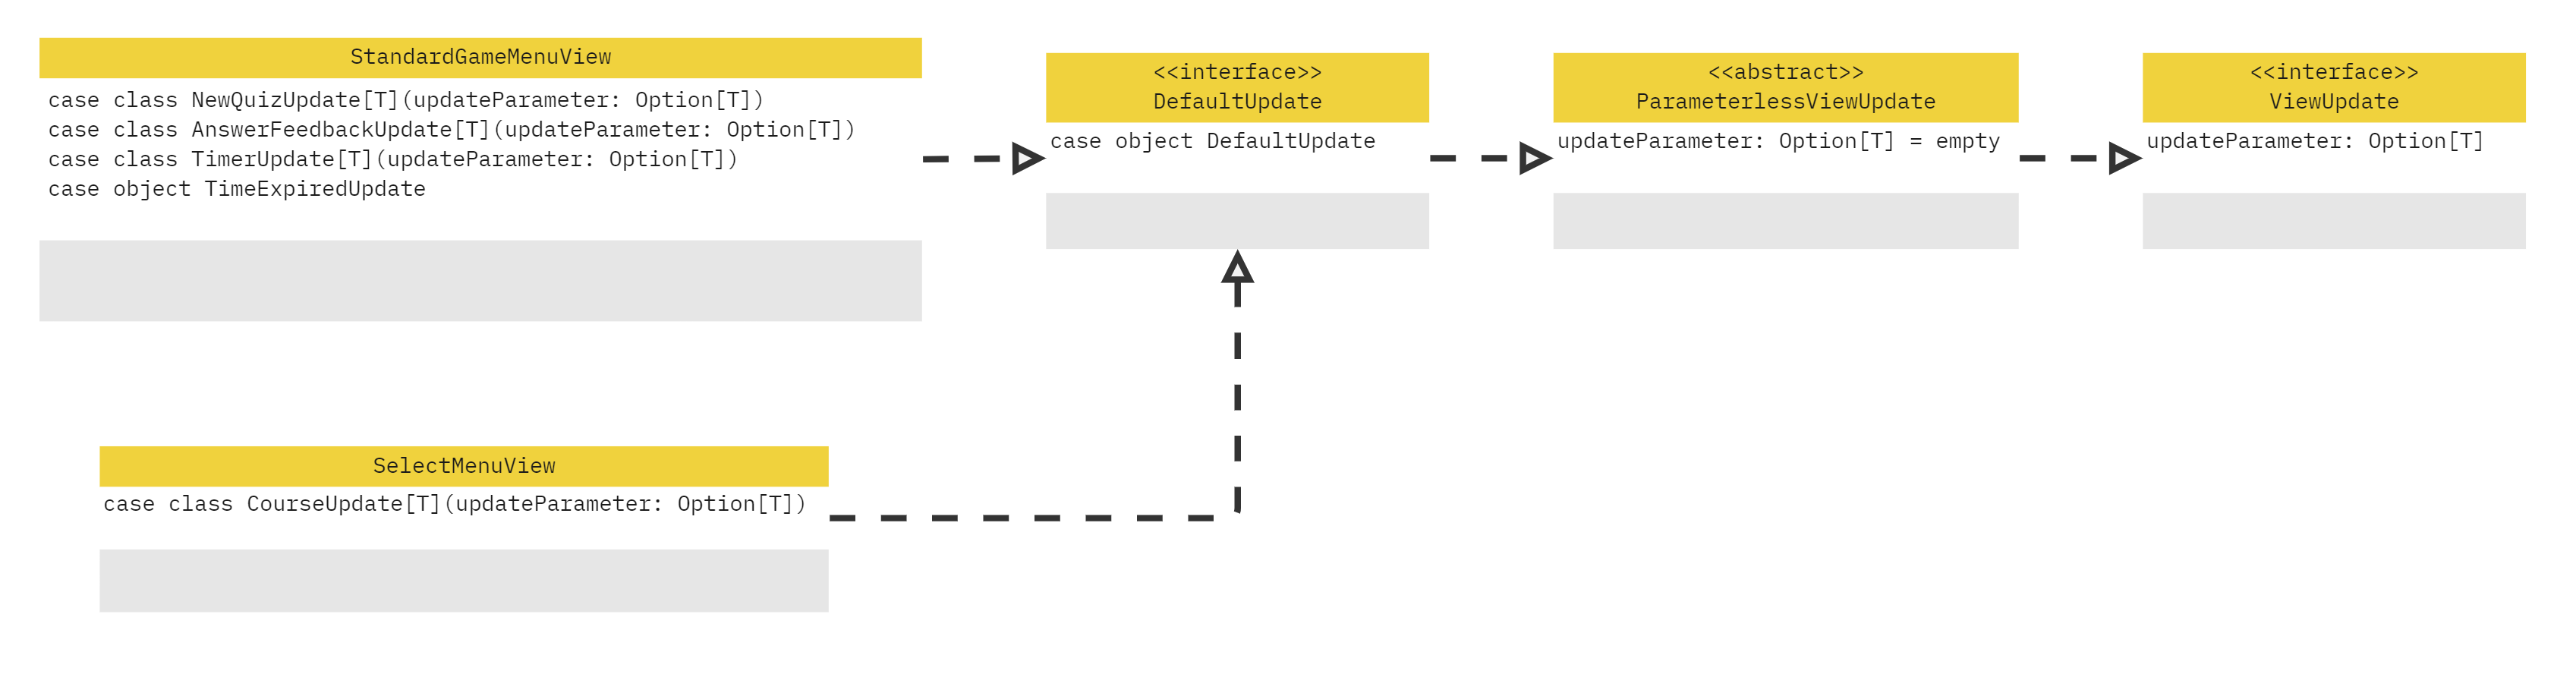
\includegraphics[width=\textwidth]{Miro/updates_view.png}
        \caption{Updates della \textit{view}}
        \label{fig:view-updates}
    \end{figure}
    
    \section{Controller}

    Per quanto riguarda il \textit{controller}, sono stati definiti molteplici \textit{controller}, uno per ciascuna pagina analogamente analogo alla \textit{view}. Come infatti si può notare da Figura \ref{fig:controller-page}, sono presenti un "SelectMenuController" e "StandardGameController" relativi rispettivamente alle pagine di selezione corsi e di una partita in modalità standard. Per come è stato concepito, il \textit{controller} è completamente indipendente dall'implementazione specifica dell'interfaccia grafica, come già indicato nel capitolo Architettura Generale \ref{chap:generic-controller}. 
    
    \begin{figure}[H]
        \centering
        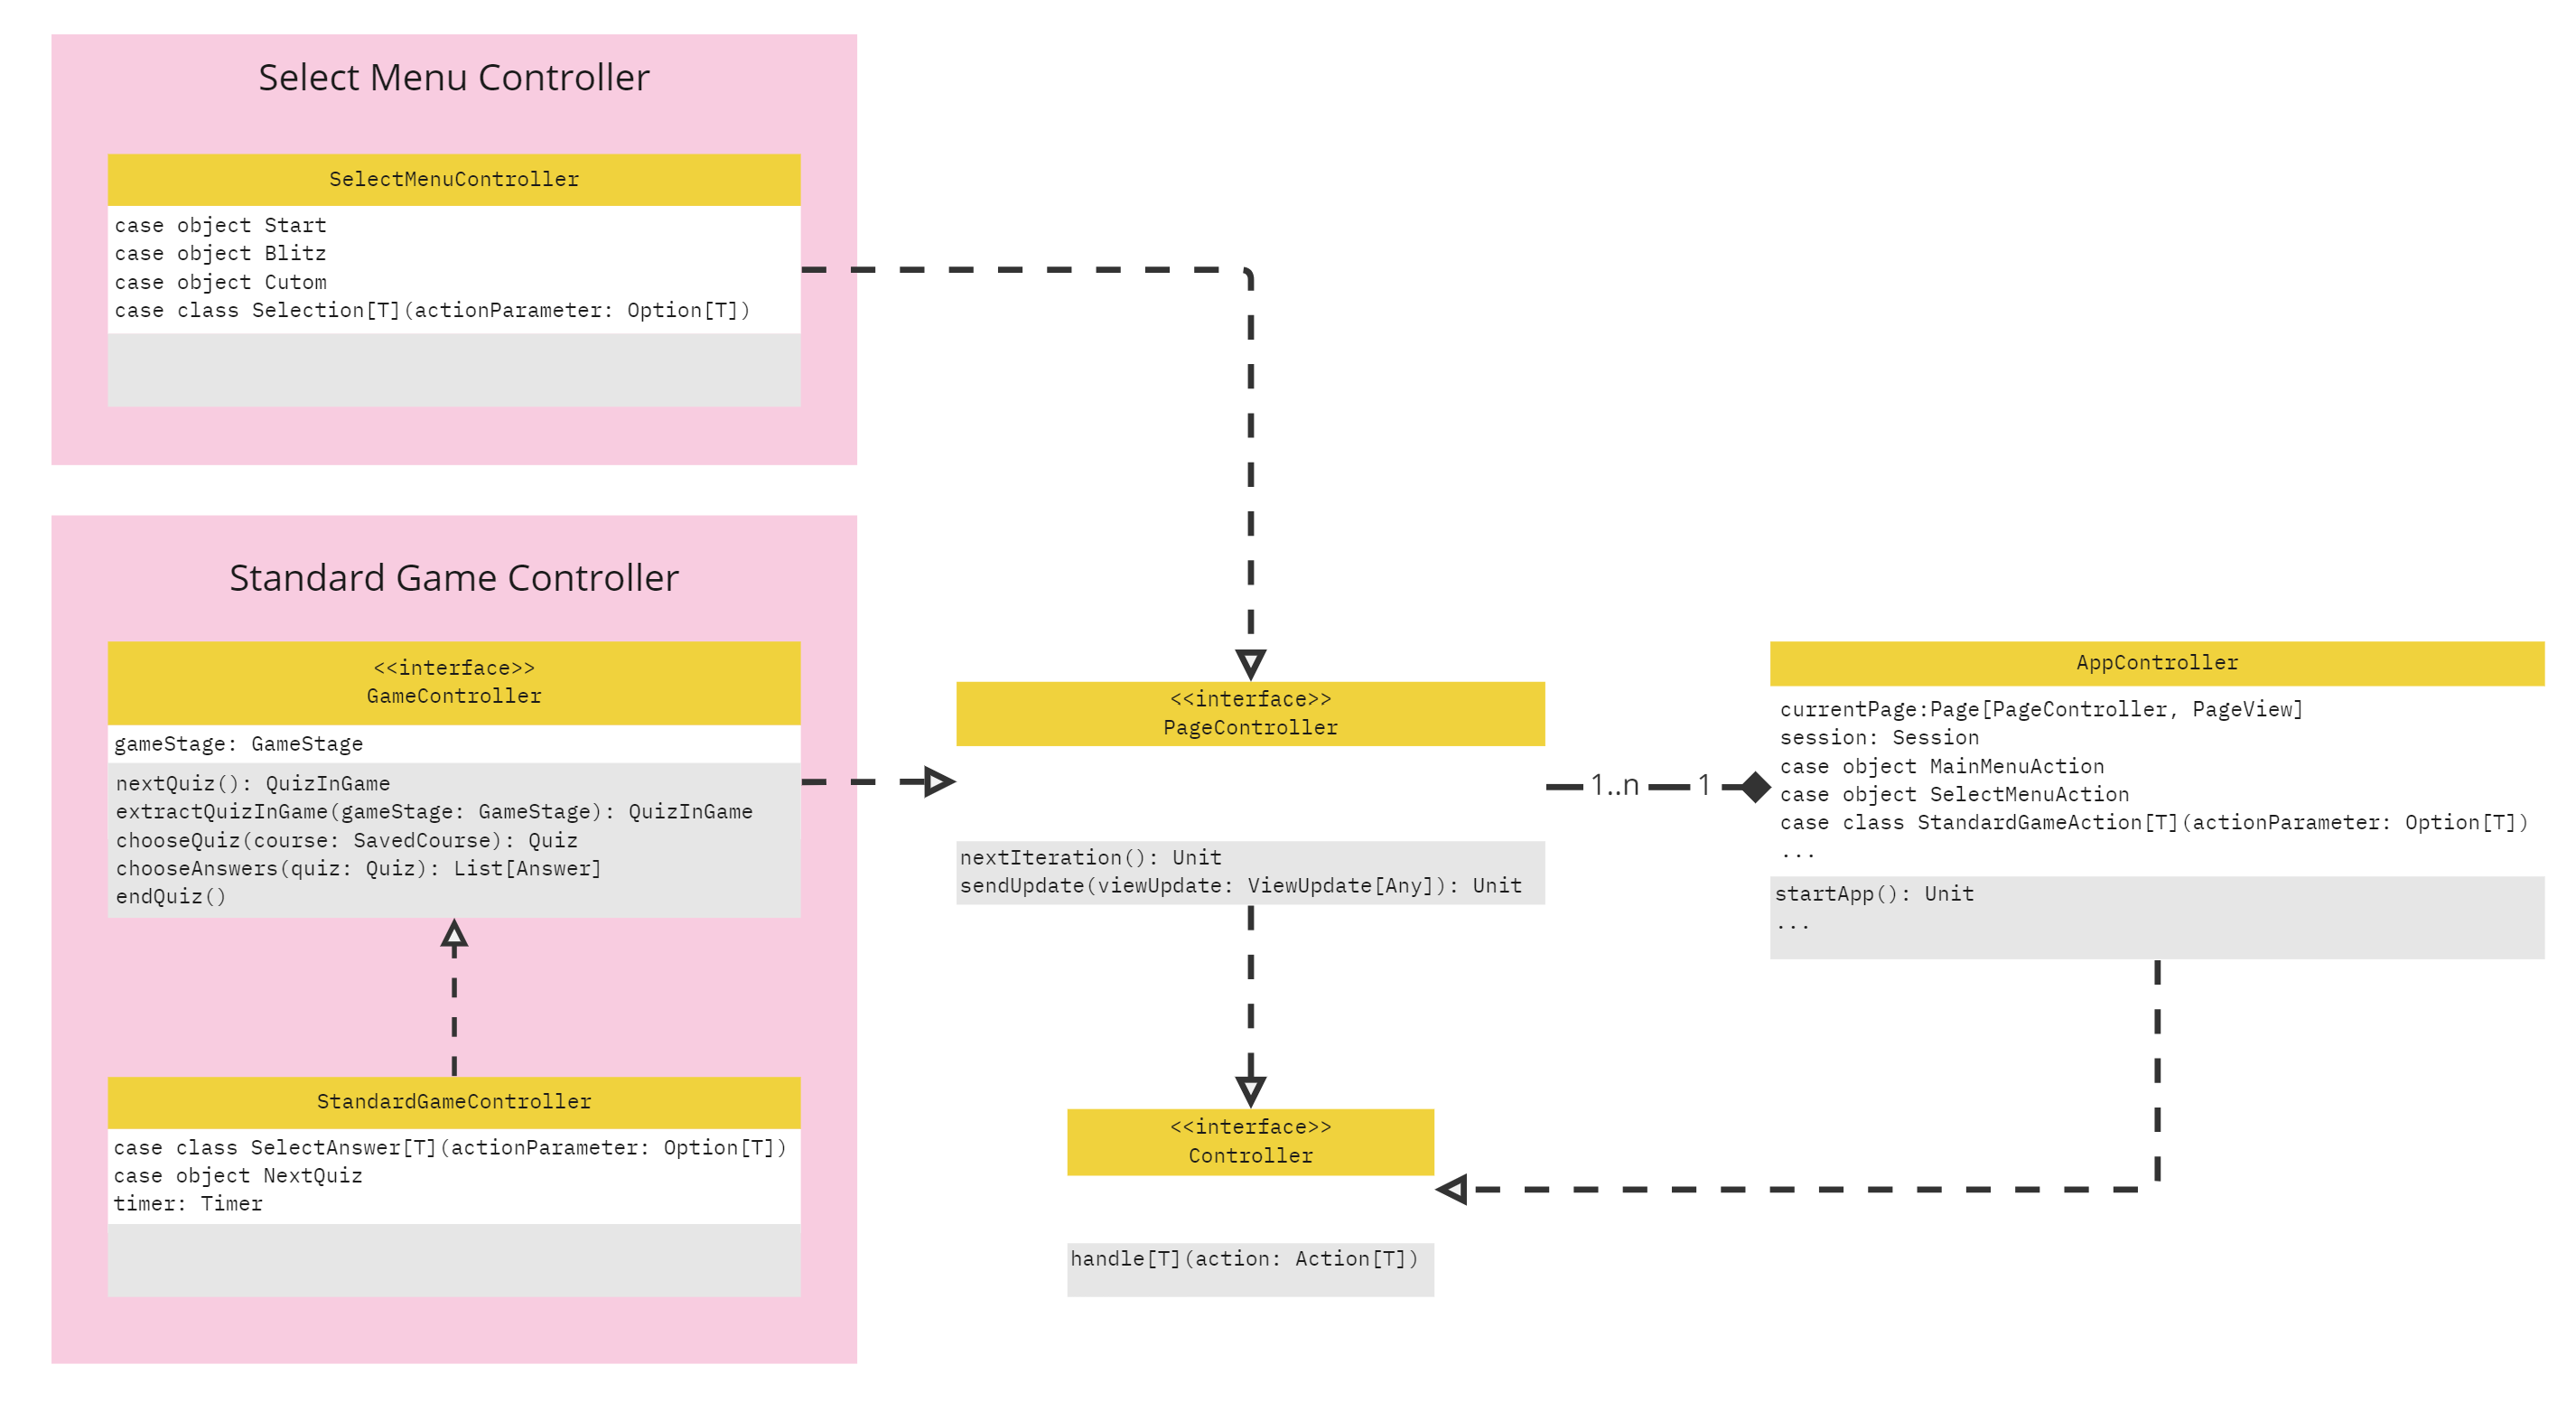
\includegraphics[width=\textwidth]{Miro/page_controller.png}
        \caption{Architettura del \textit{controller}}
        \label{fig:controller-page}
    \end{figure}

    Come per la \textit{view}, il \textit{controller} mette a disposizione una serie di azioni che l'utente può eseguire e che vengono gestite dal \textit{controller} della pagina. Una "Action" generale può portare con sé dei parametri generici ed opzionali o averli vuoti nel caso si tratti di una "ParameterLessAction", ovvero di una azione senza parametri aggiuntivi. Anche in questo caso le parti in comune tra i vari \textit{controller} sono state estratte così come nell'esempio di Figura \ref{fig:controller-actions}, dove è mostrata la "BackAction" che rappresenta un'azione generica per tornare alla pagina precedente.
    
    \begin{figure}[H]
        \centering
        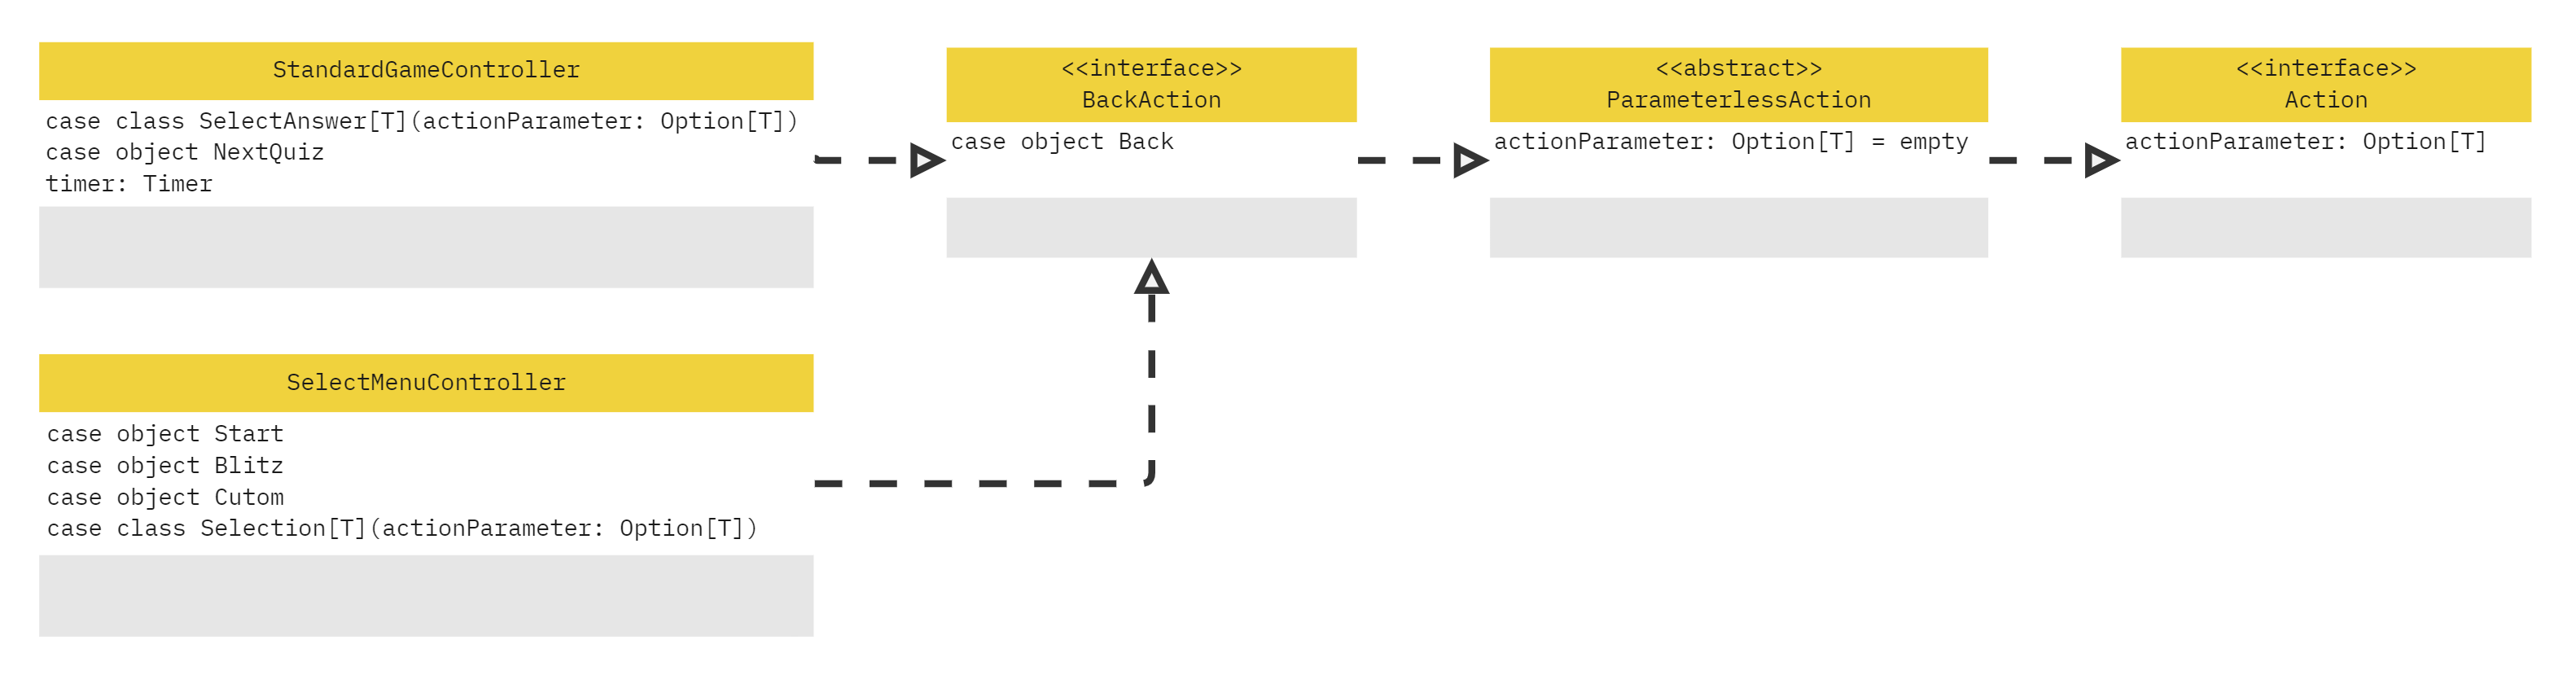
\includegraphics[width=\textwidth]{Miro/actions_controller.png}
        \caption{Actions del \textit{controller}}
        \label{fig:controller-actions}
    \end{figure}

    Come già specificato, la comunicazione tra il  \textit{view} e il \textit{controller} di una pagina avviene solamente attraverso le "Action" e i "ViewUpdate", nello specifico: la  \textit{view} invia al controller le azioni eseguite da un utente attraverso le "Action" specifiche definite e gestite da quel \textit{controller}, mentre il \textit{controller} manda alla \textit{view} gli update che l'interfaccia grafica è in grado di visualizzare.
    